\subsection{Kiến trúc Network: }
\label{sec:network-archi}
Ở phần này chúng tôi sẽ giới thiệu các thành phần cơ bản của Network. \\

\begin{figure}[H]
	\centering
	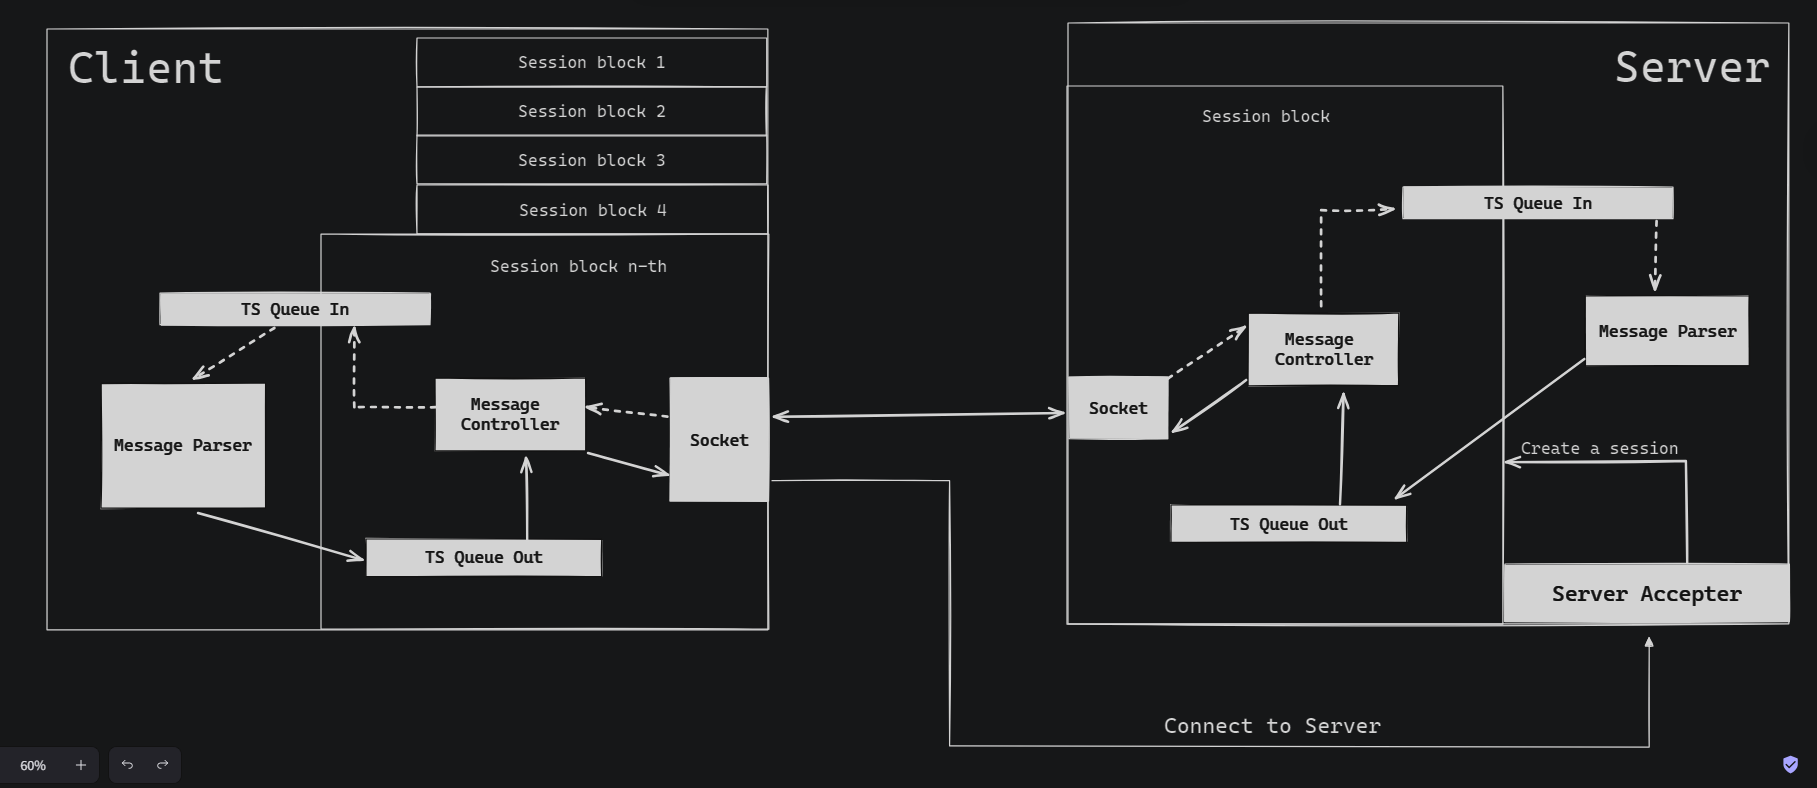
\includegraphics[width=\linewidth]{latex/architechture/architechture_diagram.png}
	\caption{Networking Architechture Diagram}
	\label{fig:network}
\end{figure}

Trên đây là mô hình cơ bản của kiến trúc network của chúng tôi và luồng di chuyển của message. Lưu ý: ở đây với mũi tên vẽ liền đại diện cho luồng di chuyển message \textit{ra ngoài}, còn mũi tên nét đứt đại diện cho message được gởi \textit{vào}.

\subsubsection{Message: }
\label{sec:message}
\textbf{Message} là dữ liệu cơ bản được truyền đi nhằm thực hiện giao tiếp giữa hai ứng dụng với nhau.

Kiểu dữ liệu được thiết kế gồm hai phần:
\begin{itemize}
	\item \textbf{Header} chứa những thông tin cơ bản của message, ở đây là \underline{kích cỡ message} và \underline{loại message}, chi tiết về \underline{các loại message} sẽ được trình bày tại phần 
	\textbf{\hyperref[subsec:Protocol]{Thiết kế Protocol}}.
	\item \textbf{Body} chứa \underline{toàn bộ dữ liệu của message}.
\end{itemize}

Việc thiết kế thêm phần Header sẽ giúp cho việc giao tiếp giữa hai ứng dụng trở nên dễ dàng phân loại và quản lý hơn.

\subsection{ThreadSafe Queue: }

Là một kiểu dữ liệu quan trọng trong cấu trúc ứng dụng, được thiết kế để giải quyết tính tuần tự của các sự kiện, kết nối, message....  đảm bảo an toàn khi truy cập dữ liệu, không xảy ra mâu thuẫn, thiếu sót và tối ưu hóa việc sử dụng tài nguyên trong quá trình xử lý đa luồng của máy tính.

Kiểu dữ liệu này bản chất là một hàng đợi hai đầu, nhưng được tích hợp thêm khoá \textit{(Mutex)} và cơ chế \textit{Wait}, cụ thể như sau :
\begin{itemize}
	\item \textbf{Mutex} : Ở mỗi thao tác có sự tác động tới dữ liệu trong \textit{Queue}, chúng đều sẽ khoá \textit{Mutex} chung lại, đảm bảo rằng chỉ sau khi xử lý xong công việc mới được tiếp tục đi tới thao tác tác động tới dữ liệu khác, điều này đảm bảo tính nhất quán của dữ liệu trong \textit{Queue}, tránh mâu thuẫn và xung đột khi nhiều luồng cùng truy cập. Điều này rất quan trọng để đảm bảo an toàn khi xử lý đa luồng.
	\item \textbf{Cơ chế Wait} : nhằm tiết kiệm tài nguyên của máy tính, \textit{Queue} sẽ được đưa vào trạng thái chờ đợi \textit{(không sử dụng tài nguyên)} nếu nó rỗng, và chỉ trở lại hoạt động khi một phần tử mới được thêm vào.
\end{itemize}

\underline{Lưu ý}: ThreadSafe Queue được sử dụng cho mọi hàng đợi được tạo ra trong phần Network, vì thế để thuận tiện, kể từ bây giờ chúng tôi sẽ gọi là \textit{Hàng đợi} (\textit{Queue}) và ngầm hiểu đó là đối tượng \textit{ThreadSafe Queue}.

\subsubsection{Session: }
\textbf{Session} là thành phần chính của kiến trúc mạng của chúng tôi. Thành phần này được thiết kế như là nơi thực hiện việc giao tiếp trực tiếp với đối tượng bên ngoài thông qua socket. Mỗi session sẽ chỉ tạo với mỗi kết nối được thiết lập giữa \textit{Client} và \textit{Server} và được dùng để giao tiếp giữa chính hai đối tượng đó. Điều này giúp việc quãn lý bộ nhớ và các trạng thái một cách dễ dàng và tự động, giảm độ phức tạp trong việc xử lý gởi nhận trong quá trình giao tiếp.

Session chứa các đối tượng chính như là: 
\begin{itemize}
	\item \textbf{Socket} - Endpoint cho kết nối. Trong kiến trúc mạng của chúng tôi, chỉ session mới chứa socket để thực hiện giao tiếp.
	\item \textbf{IncomingQueue} - Hàng đợi message cho dữ liệu được nhận vào, được thiết kế là một đối tượng std::shared\_ptr và được tham chiếu bởi cả \textit{Session} và đối tượng chứa nó (\textit{Client} hoặc \textit{Server}). Khi \textit{Session} nhận được message từ bên ngoài, đối tượng này sẽ kiểm tra tính hợp lệ của message (theo phong cách đã được định nghĩa), sau đó sẽ được đưa vào xử lý bởi \textit{Client} và \textit{server}. Điều này giúp làm tránh các xung đột và những bất cập trong việc quãn lý khi một server có thể xử lý nhiều \textit{Session}. Khi đó, các đối tượng như \textit{Server} hay \textit{Client} có thể dễ dàng xử lý trong một hàng đợi duy nhất và gởi đi message mới cho đúng \textit{Session}.
	\item \textbf{OutcomingQueue} - Hàng đợi message cho dữ liệu gởi đi. Khác với \textit{IncomingQueue}, \textit{OutcomingQueue} chỉ được tham chiếu bởi \textit{Session}. Trong khi kết nối được thiết lập, \textit{Session} sẽ luôn kiểm tra \textit{OutcomingQueue} còn dữ liệu không, nếu có sẽ gởi tất cả những dữ liệu bên trong và đợi cho đến khi có message mới được thêm vào.
\end{itemize}

\subsubsection{IClient và IServer: }
\textit{IClient} và \textit{IServer} là hai abstract class tạo ra để quãn lý, phân phối và xử lý các event và message.  \\
Trong \textit{IClient} và \textit{IServer} đều được thiết kế các hàm để kết nối, chấp nhận kết nối, gởi và nhận các message từ \textit{Session} và quãn lý các \textit{Session} này. \textit{Client} và \textit{Server} chứa một hàng đợi gọi là \textit{IncomingQueue} như hình trên đã thể hiện. Chúng có nhiệm vụ nhận các message từ \textit{Session} và phân phối và xử lý dựa trên HeadID của message mà phân phối cho các handler phù hợp. \\
Trong cách implementation của mình, chúng tôi chỉ cho các class này tạo ra 2 \textit{Session} mỗi kết nối, một cho việc truyền dữ liệu ảnh từ \textit{Server} sang \textit{Client}, một dành cho việc truyền các event điều khiển từ \textit{Client} sang \textit{Server}. Việc này giúp dữ liệu ở \textit{Session} không bị tràn khi mà kích thước dữ liệu ảnh sẽ khá lớn. 


Một vài điểm khác biệt giữa Client và Server ở đây: 
\begin{itemize}
	\item \textbf{IServer: } Là đối tượng được phía \textbf{Client} kết nối đến và điều khiển từ xa. \textit{IServer} chứa các đối tượng acceptor của thư viện ASIO, nhằm \textit{accept} các kết nối từ \textit{Client}. Để tránh các xung đột không cần thiết, chúng tôi đã thiết kế mỗi một Server chỉ tạo duy nhất một kết nối với một Client.
	\item \textbf{IClient: } Là đối tượng được dùng để điều khiển máy từ xa hay cụ thể ở đây chính là \textit{Server}. 
\end{itemize}

\subsubsection{Giao tiếp giữa các thành phần: }

\textbf{a. Thiết lập kết nối:}
\begin{figure}[H]
	\centering
	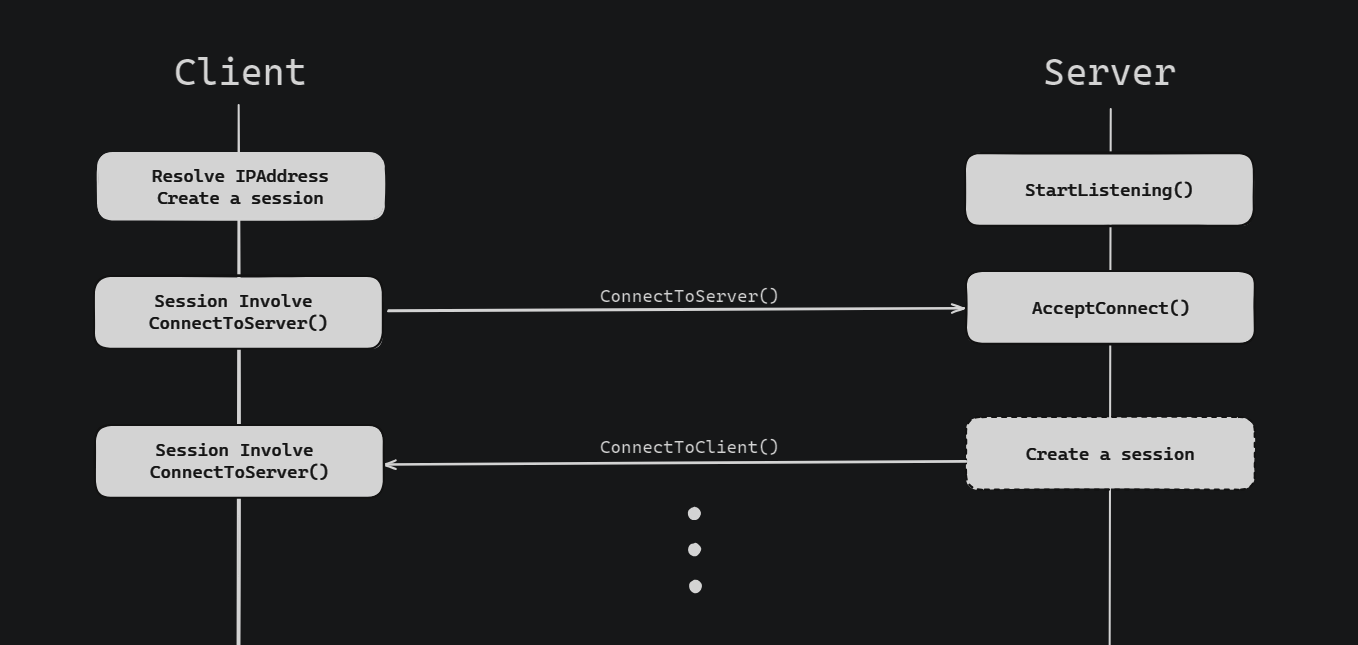
\includegraphics[width=\linewidth]{latex/architechture/connecting}
	\caption{Establish connection}
	\label{fig:handshake}
\end{figure}

\textbf{b. Nhận và gởi: }
Sơ đồ \ref{fig:network} cũng đã mô tả quá trình giao tiếp giữa các thành phần trong mạng với nhau. 
\begin{itemize}
	\item Ở quá trình \textbf{gởi}: Sau khi message được tạo bởi \textit{Client} hoặc \textit{Server}, message sẽ được kiểm tra đưa vào đúng \textit{Session} cần gởi. Message khi vào \textit{Session} sẽ được đưa vào \textit{OutcomingQueue} để chờ các gói message phía trước nó được gởi. Khi đến lượt, message sẽ được gởi thông qua hai giai đoạn: \textit{WriteHeader()} gởi Header và \textit{WriteBody()} gởi Body bằng \textit{Socket}. Việc này sẽ làm giảm sức ép lên băng thông và vẫn đảm bảo nhận đủ dữ liệu khi mà kích thước của Header là cố định còn kích thước Body đã được lưu trữ ở Header.
	\item Ở quá trình \textbf{Nhận}: Khi nhận, \textit{socket} của \textit{Session} bên nhận sẽ là nơi xử lý đầu tiên, lặp lại đúng như thứ tự gởi ở bên gởi. \textit{ReadHeader()} và \textit{ReadBody()}. Khi quá trình nhận hoàn thành, message mới sẽ được tạo và sẽ được đẩy vào \textit{IncomingQueue} để \textit{Client} hoặc \textit{Server} để xử lý.
\end{itemize}

\subsection{Thiết kế Protocol: }

Tại phần này, chúng tôi sẽ trình bày chi tiết giao thức mà Client và Server dùng để giao tiếp với nhau. 

\subsubsection{Thiết lập kết nối, cập nhật và ngắt kết nối}

\begin{itemize}
	\item \textbf{Kết nối: } Sau khi \textbf{Client} được khởi tạo và yêu cầu kết nối với \textbf{Server} đang \textit{Listening}, nếu yêu cầu được chấp nhận, \textbf{Server} sẽ phản hồi bằng cách gửi một \textit{message} có kiểu header là \textbf{SERVER\_ACCEPT}. \textbf{Client} nhận được phản hồi này và tiến hành xử lý các bước khởi tạo, hoàn tất việc thiết lập kết nối giữa hai bên.
	\item \textbf{Cập nhật: } Trong quá trình kết nối, cả hai đều liên tục trao đổi thông tin. Về phía \textbf{Server}, nó sẽ gửi các thông tin cập nhật đến màn hình Remote của \textbf{Client}, mỗi thông tin này đều được gửi dưới các \textit{message} có kiểu header là \textbf{SERVER\_UPDATE}. Về phía \textbf{Client}, có nhiều loại \textit{message} khác nhau được sử dụng để cập nhật thông tin cho \textbf{Server}. Chúng sẽ được mô tả chi tiết trong các phần tiếp theo của \textbf{Kiến trúc Protocol}.
	\item \textbf{Ngắt kết nối}Khi \textbf{Server} chủ động ngắt kết nối, nó sẽ gửi thông báo cho \textbf{Client} qua \textit{message} có kiểu header là \textbf{SERVER\_DISCONNECT}, nội dung rỗng. Tương tự, nếu \textbf{Client} chủ động ngắt kết nối, nó cũng sẽ gửi thông báo cho \textbf{Server} qua \textit{message} có kiểu header là \textbf{CLIENT\_DISCONNECT}.
\end{itemize}
	
\subsubsection{MetaData}

Giao tiếp này giúp người dùng bên \textbf{Client} và \textbf{Server} nhận được các thông tin cơ bản của nhau.

Khi \textbf{Client} được tạo, nó sẽ ngay lập tức gọi hàm để gửi các thông tin như \textit{địa chỉ IP, địa chỉ MAC},... cho \textbf{Server}, với \textit{message header} là \textbf{MetaData}.

Về phía \textbf{Server}, nó cũng sẽ gửi các thông tin cơ bản. Các thông tin này được gửi đi cùng với \textit{message} có  \textit{header} là \textbf{SERVER\_ACCEPT} đã được trình bày ở trên.

\subsubsection {Các sự kiện chuột, bàn phím}

Nội dung được trình bày sau đây là các loại \textit{message} chứa sự kiện chuột, bàn phím mà \textbf{Client} gửi tới \textbf{Server}.

Để thông tin được trình bày một cách rõ ràng và khái quát nhất, sau đây tôi sẽ liệt kê từng loại \textit{message header}, miêu tả thành phần nội dung được lưu trữ của \underline{tin nhắn mang header đó} và \underline{công việc của loại tin nhắn} đó.

\begin{itemize}
	\item \textbf{MouseClick}:  Dùng để gửi sự kiện chuột được nhấn. Chứa toạ độ tung, hoành nơi mà \textbf{Client} ấn chuột và loại nút chuột được nhấn \textit{(left, right, middle, aux1...)}.
	\item \textbf{MouseUnClick}: Dùng để gửi sự kiện chuột được nhả ra. Cũng chứa toạ độ và loại nút chuột được nhả.
	\item \textbf{DoubleClick}: Dùng để gửi sự kiện double-click được nhấn. Tương tự, chứa toạ độ và loại nút.
	\item \textbf{MouseMove}: Dùng để cập nhật vị trí con trỏ chuột. Loại tin nhắn này chỉ chứa toạ độ của chuột.
	\item \textbf{MouseWheel}: Dùng để cập nhật con lăn chuột. Chứa toạ độ và một giá trị chỉ hướng lăn của chuột.
	\item \textbf{KeyPress}: Dùng để gửi sự kiện phím được nhấn. Chỉ chứa một giá trị, đó là mã của phím.
	\item \textbf{KeyRelease}: Dùng để gửi sự kiện phím được nhả. Tương tự, chứa mã của phím.
\end{itemize}

\subsection{Capture màn hình}

Để phục vụ cho chức năng \textit{Chụp màn hình Server}, hai loại \textit{message header} \textbf{CaptureRequest} và \textbf{CaptureSend} được sử dụng.

Trong đó, khi \textbf{Client} thực thi sự kiện yêu cầu ảnh chụp màn hình từ \textbf{Server}, nó sẽ gửi một \textit{message} dưới \textit{header} \textbf{CaptureRequest}. Khi gửi lại hình cho đối phương, \textbf{Server} sẽ sử dụng \textit{header} \textbf{CaptureSend}  và nội dung của tin nhắn sẽ là mảng \textit{bit} của hình được chụp.




\subsection{Kiến trúc ứng dụng: }

Ngoài kiến trúc Network đã xây dựng, chúng tôi còn xây dựng thêm các thành phần khác cho ứng dụng nhầm hỗ trợ thêm nhiều tính năng khác:

\subsubsection{Model: }
\textit{Model} là nơi định nghĩa các đối tượng user và các thuộc tính, thao tác trên đối tượng đó. Ở đây, chúng tôi định nghĩa hai loại \textit{Model} đó là: \textit{Admin} và \textit{User}. \\
Mỗi loại \textit{Model} sẽ quy định cách thức hoạt động cho cả ứng dụng sau này khi mà \textit{Admin} có chức năng điều khiển, còn \textit{User} là người dùng được điều khiển bởi \textit{Admin}. \\
Chúng tôi đã thiết kế một vài công cụ cho \textit{Model} nhằm chức năng đăng nhập, xác thực người dùng, phân quyền người dùng, và quãn lý các User cho \textit{Admin},...


\subsubsection{User Interface: }
Thiết kế giao diện căn bản cho người dùng bằng cách phân chia thành nhiều window khác nhau như: \textbf{LoginWindow}, \textbf{MainWindow}, \textbf{CaptureWindow},...

\subsection{Nhận xét: }

\textbf{Ưu điểm: }
\begin{itemize}
	\item \textbf{Phân chia rõ ràng và độc lập}: Kiến trúc được phân chia thành các thành phần như Message, ThreadSafe Queue, Session, IClient và IServer, Giao tiếp giữa các thành phần, giúp chúng hoạt động một cách độc lập và giảm sự phụ thuộc lẫn nhau. Điều này tạo điều kiện thuận lợi cho việc phát triển, giảm thời gian kiểm tra lỗi và sửa lỗi.
	\item \textbf{Quản lý bộ nhớ và trạng thái tự động}: Session được thiết kế để quản lý bộ nhớ và trạng thái một cách tự động, giúp giảm độ phức tạp trong việc xử lý gửi nhận trong quá trình giao tiếp.
	\item \textbf{Hàng đợi ThreadSafe:} Sử dụng ThreadSafe Queue cho mọi hàng đợi tạo ra trong phần Network, giúp đảm bảo an toàn khi truy cập từ nhiều luồng thực thi khác nhau.
	\item \textbf{Quá trình phát triển: } Giúp việc phát triển dễ dàng và nhanh chóng hơn, giảm thời giam kiểm lỗi và sửa lỗi. Việc giảm thiểu sự phụ thuộc giữa các thành phần giúp dễ dàng mở rộng ứng dụng và thêm nhiều tính năng hơn khi quá trình sửa chữa và thay thế trên ít file hơn.
\end{itemize}

\textbf{Khuyết điểm: }
\begin{itemize}
	\item \textbf{Hạn chế do giới hạn kết nối}: Hiện tại, chúng tôi chỉ thiết kế duy nhất hai \textit{Session} cho mỗi Client và Server. Điều này có thể khiến cho vài tính năng khó có thể được hiện thực hóa hơn. 
	\item \textbf{Giới hạn về tốc độ}: Việc sử dụng Session chung với giao thức TCP có thể làm chậm hơn quá trình gởi nhận ảnh khi yêu cầu của người dùng là real-time. Chúng tôi đã từng xem xét đến việc sử dụng UDP cho ứng dụng. Tuy nhiên, ứng dụng được sử dụng cho người dùng trong mạng LAN nên tốc độ truyền ảnh đã nằm ở mức chấp nhận được. Ngoài ra, chúng tôi nhận thấy rằng việc truyền dữ liệu đáng tin cậy mang nhiều ưu điểm hơn trong ứng dụng Remote Desktop như bảo mật, kiểm soát luồng, đảm bảo hiệu ứng xử lý hình ảnh,...
	\item \textbf{Quá trình phát triển: } Việc phân chia thành nhiều thành phần làm cho giai đoạn đầu sẽ khá phức tạp và nặng nề. Cả với những ai muốn phát triển và đóng góp cho đồ án cũng sẽ khó tiếp cận hơn. Nhưng về sau, việc phát triển sẽ dễ dàng hơn trước nhiều.
\end{itemize}



